%  ___ _         _ _        _   _
% | _ (_)____  _| | |_ __ _| |_(_)
% |   / (_-< || | |  _/ _` |  _| |
% |_|_\_/__/\_,_|_|\__\__,_|\__|_|



% Slide 7 % % % % % % % %
\begin{frame}[plain]{\alert{Risultati}}
\label{frm:risultati:1}


      Età, genere, abilità e frequenza di utilizzo di Internet non sono risultati fattori influenti
      sul comportamento di ricerca

      \begin{equation*}
        p_{s} \in \left[.07, .96 \right]
      \end{equation*}


\end{frame}

\begin{frame}[plain]{\alert{Risultati}}
  \label{frm:risultati:2}

  \begin{columns}

    % Colonna Sinistra
    \begin{column}{0.5\linewidth}
      \begin{figure}
        \resizebox {\linewidth} {!} {

\begin{tikzpicture}[font=\small]
  \begin{axis}[
      ybar,
      bar width=25pt,
      xlabel={Stile~Cognitivo},
      ylabel={Media~Revisite},
      ymin=0,
      ytick=\empty,
      xtick=data,
      axis x line=bottom,
      axis y line=left,
      enlarge x limits=0.2,
      symbolic x coords={Landmark, Route, Survey},
      xticklabel style={anchor=base,yshift=-\baselineskip},
      nodes near coords,
      scaled y ticks=false,
      every node near coord/.style={/pgf/number format/fixed}
    ]
      \addplot[fill=gray!40,  name nodes near coords=apex] coordinates {
        (Landmark, 0.900)
        (Route, 0.333)
        (Survey, 0.067)
      };
 \end{axis}
 \draw (apex-0) -- +(0,1) -- +(4.9,1) node[pos=0.5,anchor=south] {$p < 0.05$} -- (apex-last);
\end{tikzpicture}

}
 \label{fig:hist}
      \end{figure}
    \end{column}

    % Colonna destra
    \begin{column}{0.5\textwidth}
      Rispetto alla prima ipotesi, lo stile Landmark rivisita le pagine significativamente più volte
      dello stile Survey%

      \begin{equation*}
        \begin{array}{rcl}
          F_{2,27} & = & 3.87         \\
          p & < & 0.05                \\
          \eta^{2}_{p} & = & .22
        \end{array}
      \end{equation*}
    \end{column}

  \end{columns}

\end{frame}


\begin{frame}[plain]{\alert{Risultati}}
  \label{frm:risultati:3}

  Per quel che riguarda la seconda ipotesi, non emergono differenze né rispetto al tempo di navigazione
  (medio e totale, per ogni pagina e per compito) né rispetto al numero di informazioni corrette trovate%

  \begin{equation*}
    p_{s} \in \left[.32, .90\right]
  \end{equation*}

\end{frame}

% Slide 9 % % % % % % % %
\begin{frame}[plain]{\alert{Risultati}}
\label{frm:risultati:4}

  \begin{figure}
    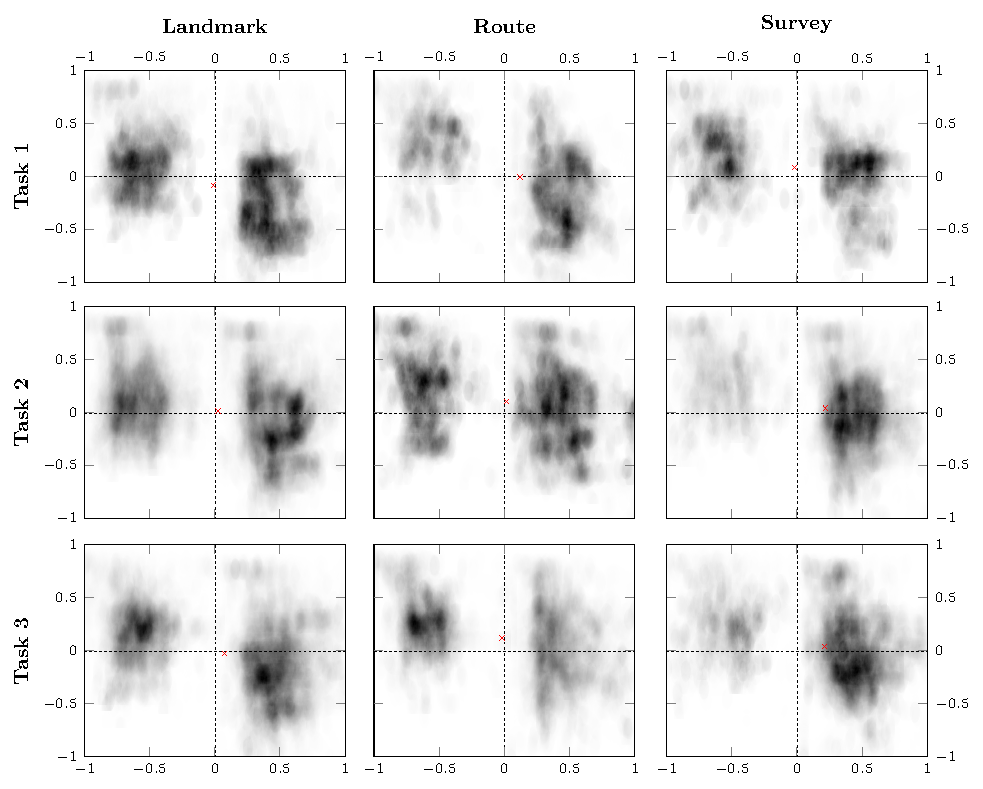
\includegraphics[height=0.8\textheight]{img/graph_2.pdf}
    \label{fig:graph_2}
  \end{figure}
\end{frame}
